\documentclass{article}

\usepackage{graphicx}
\usepackage{setspace}
\usepackage{listings}
\usepackage{color}
\usepackage{circuitikz}
\usepackage{float}

\definecolor{dkgreen}{rgb}{0,0.6,0}
\definecolor{gray}{rgb}{0.5,0.5,0.5}
\definecolor{mauve}{rgb}{0.58,0,0.82}

\lstset{basicstyle=\small,
        keywordstyle=\color{mauve},
        identifierstyle=\color{dkgreen},
        stringstyle=\color{gray},
        numbers=left
        }

\title{ECE 210 - Combinational Logic Design \\ Lab 2}
\date{2018-10-24}
\author{David Lenfesty \\ lenfesty@ualberta.ca
    \and Radomir Wasowski \\ wasowski@ualberta.ca}

\setcounter{tocdepth}{2} % Show subsections

\begin{document}

    \doublespacing
    \pagenumbering{gobble}
    \maketitle
    \newpage

    \singlespacing
    \pagenumbering{arabic}

    \section{Abstract}

    Various logic circuit designs can be combined together to create
    functional applications.

    Multiplexers and demultiplexers can be used to route specific
    incoming signals to a specified destination. In this lab a simulated
    digital signal from three different receivers was routed towards
    one of three "engineers".
    
    As well, logical elements can be used to design a simplistic access control system.
    In this lab such a circuit was designed and tested on an FPGA.

    \section{Introduction}

    The purpose of this lab was to design a simple Multiplexer and Demultiplexer circuit,
    as well as to design a circuit to control access to a lab.

    In order to validate the Multiplexer/Demultiplexer circuit,
    a useful circuit was designed using Xilinx Vivado software,
    and this circuit was simulated against the required inputs.

    In order to test the Lab Access Control circuit, the circuit was again designed
    using Xilinx Vivado, and simulated against required inputs.
    However, for this section, the design was also uploaded to a physical board
    where various inputs could be physically tested and validated.

    \section{Design Section}

    In order to design the following circuits, the Xilinx Vivado software
    was used to write VHDL that described the different logic circuits.


    \newpage
    \paragraph{MUX / DEMUX Circuit}
    In order to implement required multiplexing and demultiplexing system, the following circuit had to be implemented using VHDL.

    \begin{circuitikz}[scale=0.75, transform shape]
        \draw
            % Input selection 0
            (0,0) node[american and port](IS0){}
            (2,-1) node[american and port](sig_in_0){}
            (IS0.in 1) node[anchor=east]{S0'}
            (IS0.in 2) node[anchor=east]{S1'}
            (IS0.out) -| (sig_in_0.in 1)
            (-2,-1) node[anchor=east, color=green]{I0} -| (sig_in_0.in 2)

            % Input selection 1
            (0,-2) node[american and port](IS1){}
            (2,-3) node[american and port](sig_in_1){}
            (IS1.in 1) node[anchor=east]{S0}
            (IS1.in 2) node[anchor=east]{S1'}
            (IS1.out) -| (sig_in_1.in 1)
            (-2,-3) node[anchor=east, color=green]{I1} -| (sig_in_1.in 2)

            % Input selection 2
            (0,-4) node[american and port](IS2){}
            (2,-5) node[american and port](sig_in_2){}
            (IS2.in 1) node[anchor=east]{S0}
            (IS2.in 2) node[anchor=east]{S1'}
            (IS2.out) -| (sig_in_2.in 1)
            (-2,-5) node[anchor=east, color=green]{I2} -| (sig_in_2.in 2)

            % OR accumulation for inputs
            (4,-2) node[american or port](mux_or_1){}
            (6,-3) node[american or port](mux_or_2){}
            (sig_in_0.out) -| (mux_or_1.in 1){}
            (sig_in_1.out) -| (mux_or_1.in 2){}
            (mux_or_1.out) -| (mux_or_2.in 1){}
            (sig_in_2.out) -| (mux_or_2.in 2){}

            % Engineer 0 selection
            (2,-8)  node[american and port](eng0_sel){}
            (4,-7)  node[american and port](eng0_sig){}
            (eng0_sel.in 1) node[anchor=east]{DS0'}
            (eng0_sel.in 2) node[anchor=east]{DS1'}
            (eng0_sel.out) -| (eng0_sig.in 2){}
            (eng0_sig.out) -| (7,-7) node[anchor=west, color=red]{E0}

            % Engineer 1 selection
            (2,-10) node[american and port](eng1_sel){}
            (4,-9)  node[american and port](eng1_sig){}
            (eng1_sel.in 1) node[anchor=east]{DS0'}
            (eng1_sel.in 2) node[anchor=east]{DS1'}
            (eng1_sel.out) -| (eng1_sig.in 2){}
            (eng1_sig.out) -| (7,-9) node[anchor=west, color=red]{E1}

            % Engineer 2 selection
            (2,-12) node[american and port](eng2_sel){}
            (4,-11) node[american and port](eng2_sig){}
            (eng2_sel.in 1) node[anchor=east]{DS0'}
            (eng2_sel.in 2) node[anchor=east]{DS1'}
            (eng2_sel.out) -| (eng2_sig.in 2){}
            (eng2_sig.out) -| (7,-11) node[anchor=west, color=red]{E1}


            % Intermediate signal 'Z'
            (mux_or_2.out) node[anchor=south]{Z} -| (8,-3) -| (8,-6)
            -| (-2,-6) -| (-2,-7) -| (1,-7) -| (eng0_sig.in 1)
            (-2,-6) -- (-2,-9) -| (eng1_sig.in 1)
            (-2,-6) -- (-2,-11) -| (eng2_sig.in 1)
        ;
    \end{circuitikz}

    The folllowing VHDL architecture was written to implement this circuit in hardware.

    \begin{lstlisting}[language=VHDL]
architecture Behavioral of lab2_part1 is
    signal M   : STD_LOGIC := '0';
    signal SEL : STD_LOGIC_VECTOR (2 downto 0) := "000";
begin
    M <=   ((not S(1) and not S(0)) and I(0))
        or ((not S(1) and S(0)) and I(1))
        or (( S(1) and not S(0) ) and I(2));
    
    SEL(0) <= (not DS(1) and not DS(0));
    SEL(1) <= (not DS(1) and DS(0));
    SEL(2) <= (DS(1) and not DS(0)); 
    O(0) <= M and SEL(0);
    O(1) <= M and SEL(1);
    O(2) <= M and SEL(2);
    EI(0) <= SEL(0);
    EI(1) <= SEL(1);
    EI(2) <= SEL(2);
end Behavioral;
    \end{lstlisting}
    \newpage

    \paragraph{Lab Access Control Circuit}
    In order to implement the required access control, the following circuit was developed.

    \begin{circuitikz}[scale=0.75, transform shape]
        \draw
            % Ports for lab0 selection
            (4,0) node[american and port](lab0-card){}
            (4,-2) node[american and port](lab0-code){}
            (1,-0.275) node[american not port](not1){}
            (1,-1.725) node[american not port](not2){}

            (0,0.5) node[anchor=east]{C1} -| (lab0-card.in 1)
            (0,-0.5) node[anchor=east]{C0} -| (not1.in)
            (not1.out) |- (lab0-card.in 2)

            (0,-1.5) node[anchor=east]{K2} -| (not2.in)
            (not2.out) |- (lab0-code.in 1)
            (0,-2.5) node[anchor=east]{K0} -| (lab0-code.in 2)

            (6, -1) node[american and port](lab0-out){}
            (lab0-card.out) -| (lab0-out.in 1)
            (lab0-code.out) -| (lab0-out.in 2)

            % Ports for lab1 selection
            (4,-4) node[american and port](lab1-card){}
            (4,-6) node[american and port](lab1-code){}
            (1,-4.3) node[american not port](not1){}
            (1,-5.725) node[american not port](not2){}

            (0,-3.5) node[anchor=east]{C0} -| (lab1-card.in 1)
            (0,-4.5) node[anchor=east]{C1} -| (not1.in)
            (not1.out) |- (lab1-card.in 2)

            (0,-5.5) node[anchor=east]{K0} -| (not2.in)
            (not2.out) |- (lab1-code.in 1)
            (0,-6.5) node[anchor=east]{K2} -| (lab1-code.in 2)

            (6, -5) node[american and port](lab1-out){}
            (lab1-card.out) -| (lab1-out.in 1)
            (lab1-code.out) -| (lab1-out.in 2)

            % Outputs for lab0/1
            (lab0-out.out) -| (8,-1) node[anchor=west, color=dkgreen]{Lab0-Unlock}
            (lab1-out.out) -| (8,-5) node[anchor=west, color=dkgreen]{Lab1-Unlock}

            % Alarm gates
            (3,-12) node[american or port](alarm-card){}
            (6,-10) node[american and port](code-not){}
            (9,-11) node[american and port](alarm){}

            % Inverters for and port
            (3, -9.25) node[american not port](not3){}
            (3, -10.75) node[american not port](not4){}
            
            % Lab0 and 1 unlock routing
            (6.5,-1) -- (6.5,-7) -| (1,-7) -| (1,-9.25) -| (not3.in)
            (7, -5) -- (7,-7.5) -| (1.5,-7.5) -| (1.5, -10.75) -| (not4.in)
            (not3.out) -| (code-not.in 1)
            (not4.out) -| (code-not.in 2)

            % Card inputs
            (1,-11.5) node[anchor=east]{C1} -| (alarm-card.in 1)
            (1,-12.5) node[anchor=east]{C0} -| (alarm-card.in 2)

            % Final card inputs/outputs
            (code-not.out) -| (alarm.in 1)
            (alarm-card.out) -| (alarm.in 2)
            (alarm.out) |- (10,-11) node[anchor=west,color=red]{Alarm}

        ;
    \end{circuitikz}

    The following VHDL architecture was written to implement this circuit in hardware.

    \begin{lstlisting}[language=VHDL]
architecture Behavioral of lab2_part2 is
    signal Lab0_Correct : STD_LOGIC := '0';
    signal Lab1_Correct : STD_LOGIC := '0';
begin

    Lab0_Correct <= (C(1) and not C(0))
                and (K(0) and not K(2));
    Lab1_Correct <= (not C(1) and C(0))
                and (not K(0) and K(2));
    
    Lab0_Unlock <= Lab0_Correct;
    Lab1_Unlock <= Lab1_Correct;
    
    Alarm <= (C(1) or C(0))
         and (not Lab0_Correct and not Lab1_Correct);
end Behavioral;
    \end{lstlisting}
    \newpage

    \section{Procedure}
    In order to test that the circuit worked properly,
    both VHDL programs were simulated, and then the
    access control code was ran on a physical FPGA and verified physically,
    using buttons.

    The circuit for part one was tested using the supplied
    simulation file. The outputs were then verified against the expected truth table.

    For part two, the circuit was simulated and run against another
    supplied simulation file. It was also uploaded to an FPGA
    board, using the provided constraints, where the functionality
    of the access system was verified by using the physical buttons and switches on
    the board.


    \section{Results}

    \paragraph{Part 1}
    The VHDL design worked perfectly according to the specifications laid out.
    Below is the output from the simulation:

    \begin{figure}[H]
        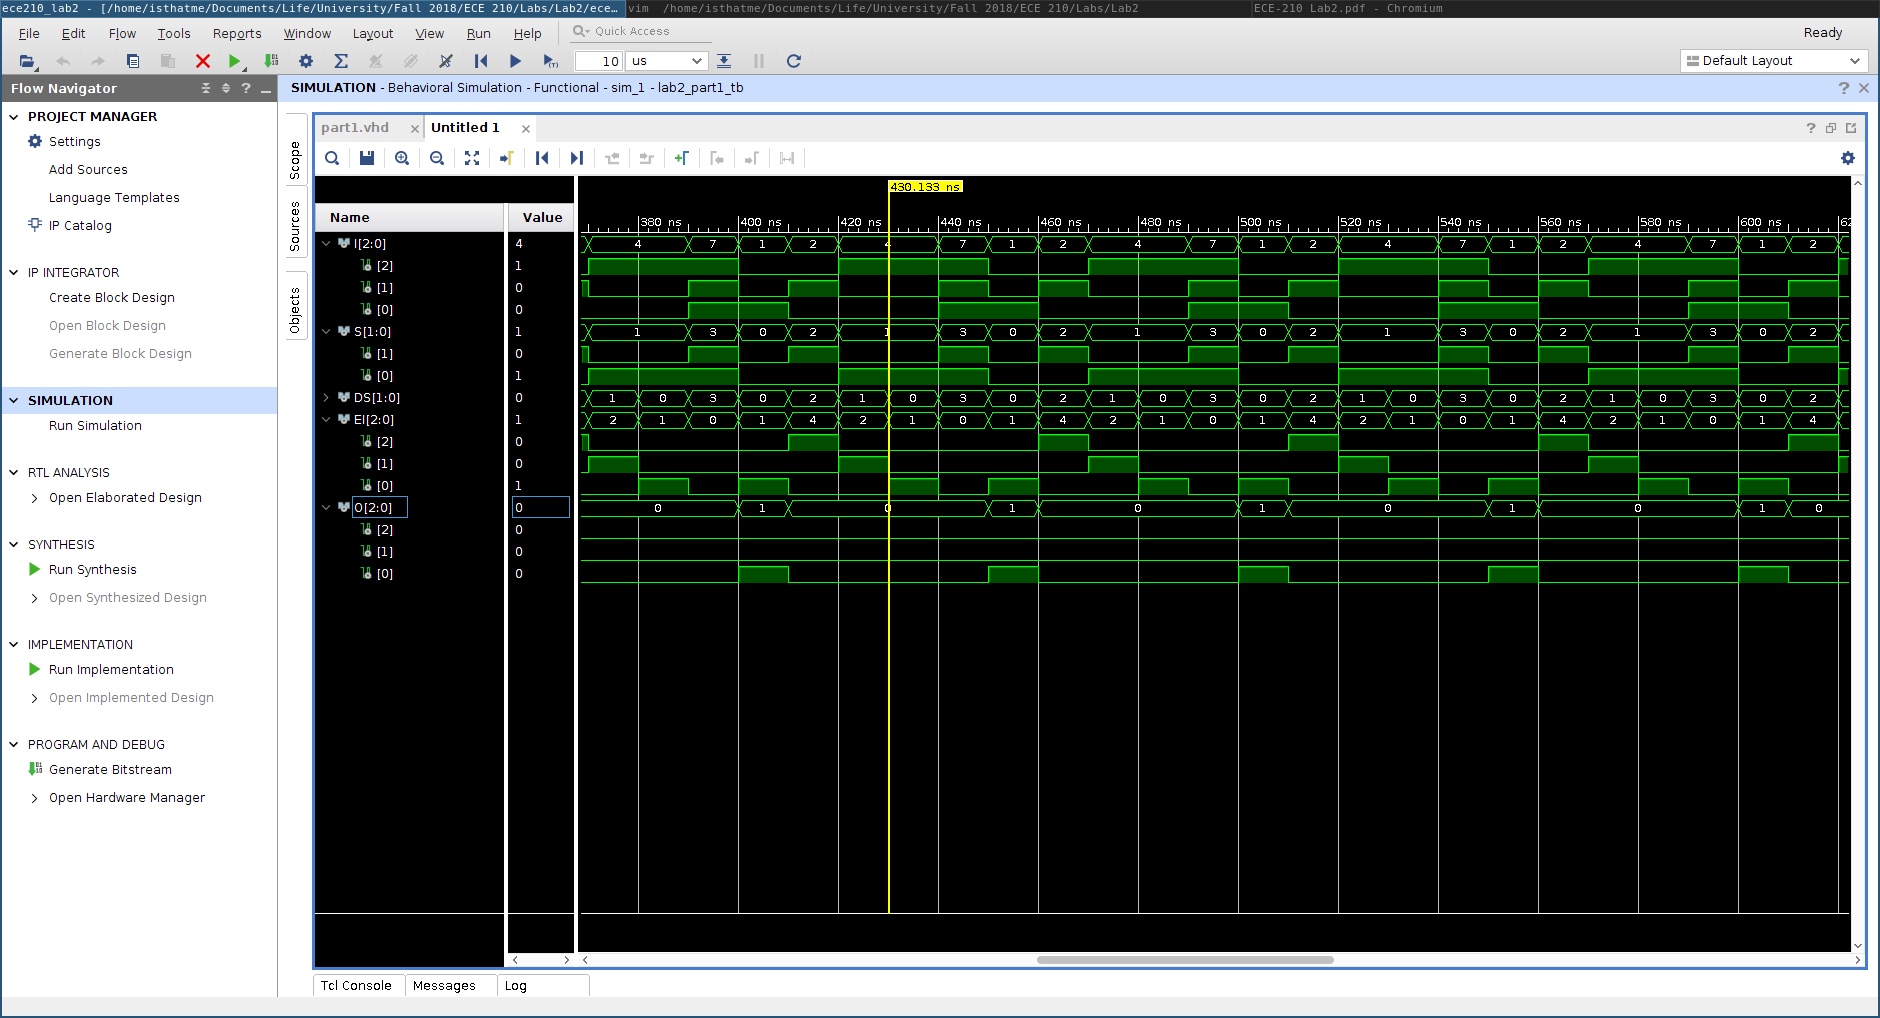
\includegraphics[width=\linewidth]{MUX_DEMUX.png}
        \caption{Part 1 Simulation}
        \label{fig:part1_sim}
    \end{figure}

    \paragraph{Part 2}
    The VHDL design was able to correctly control the lab access and alarm signals
    as specified.
    Below is an image of the simulation waveform.

    \begin{figure}[H]
        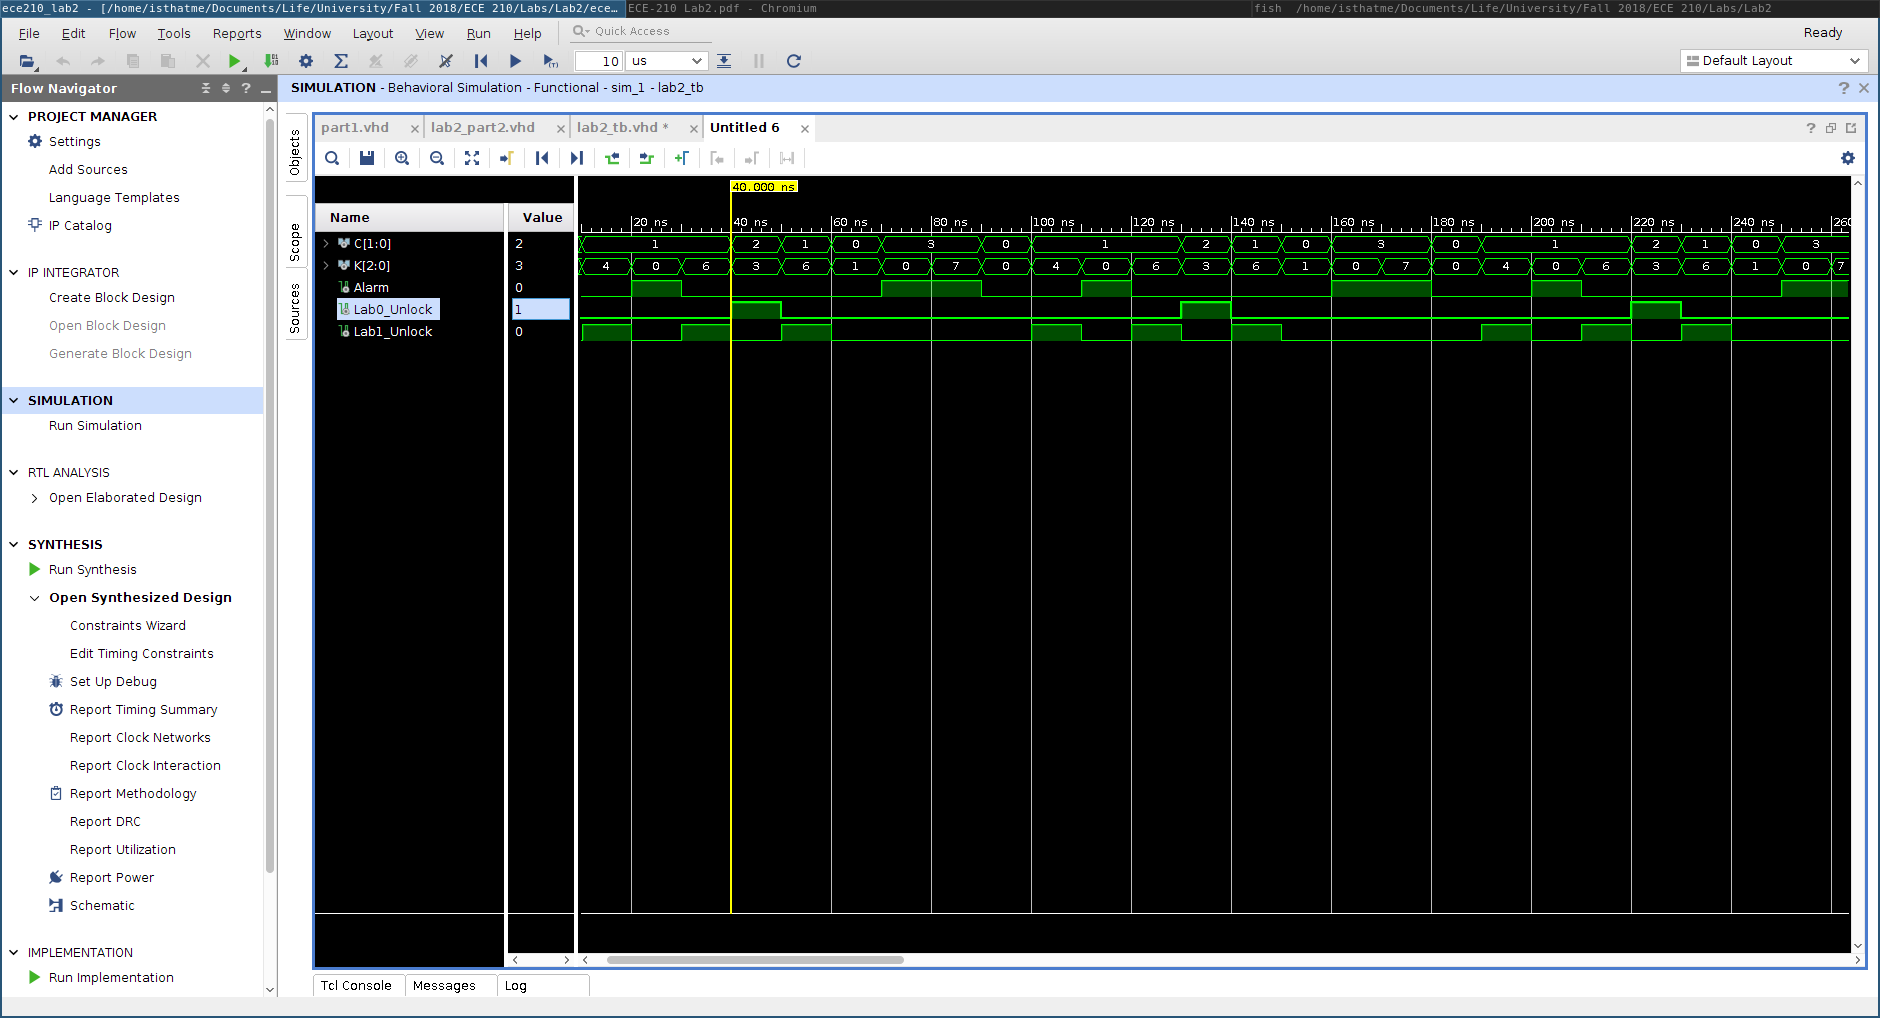
\includegraphics[width=\linewidth]{Access_control.png}
        \caption{Part 2 Simulation}
        \label{fig:part2_sim}
    \end{figure}

    Physical testing also proved to be correct.
    Below is a picture of one of the input combinations being tested.

    \begin{figure}[H]
        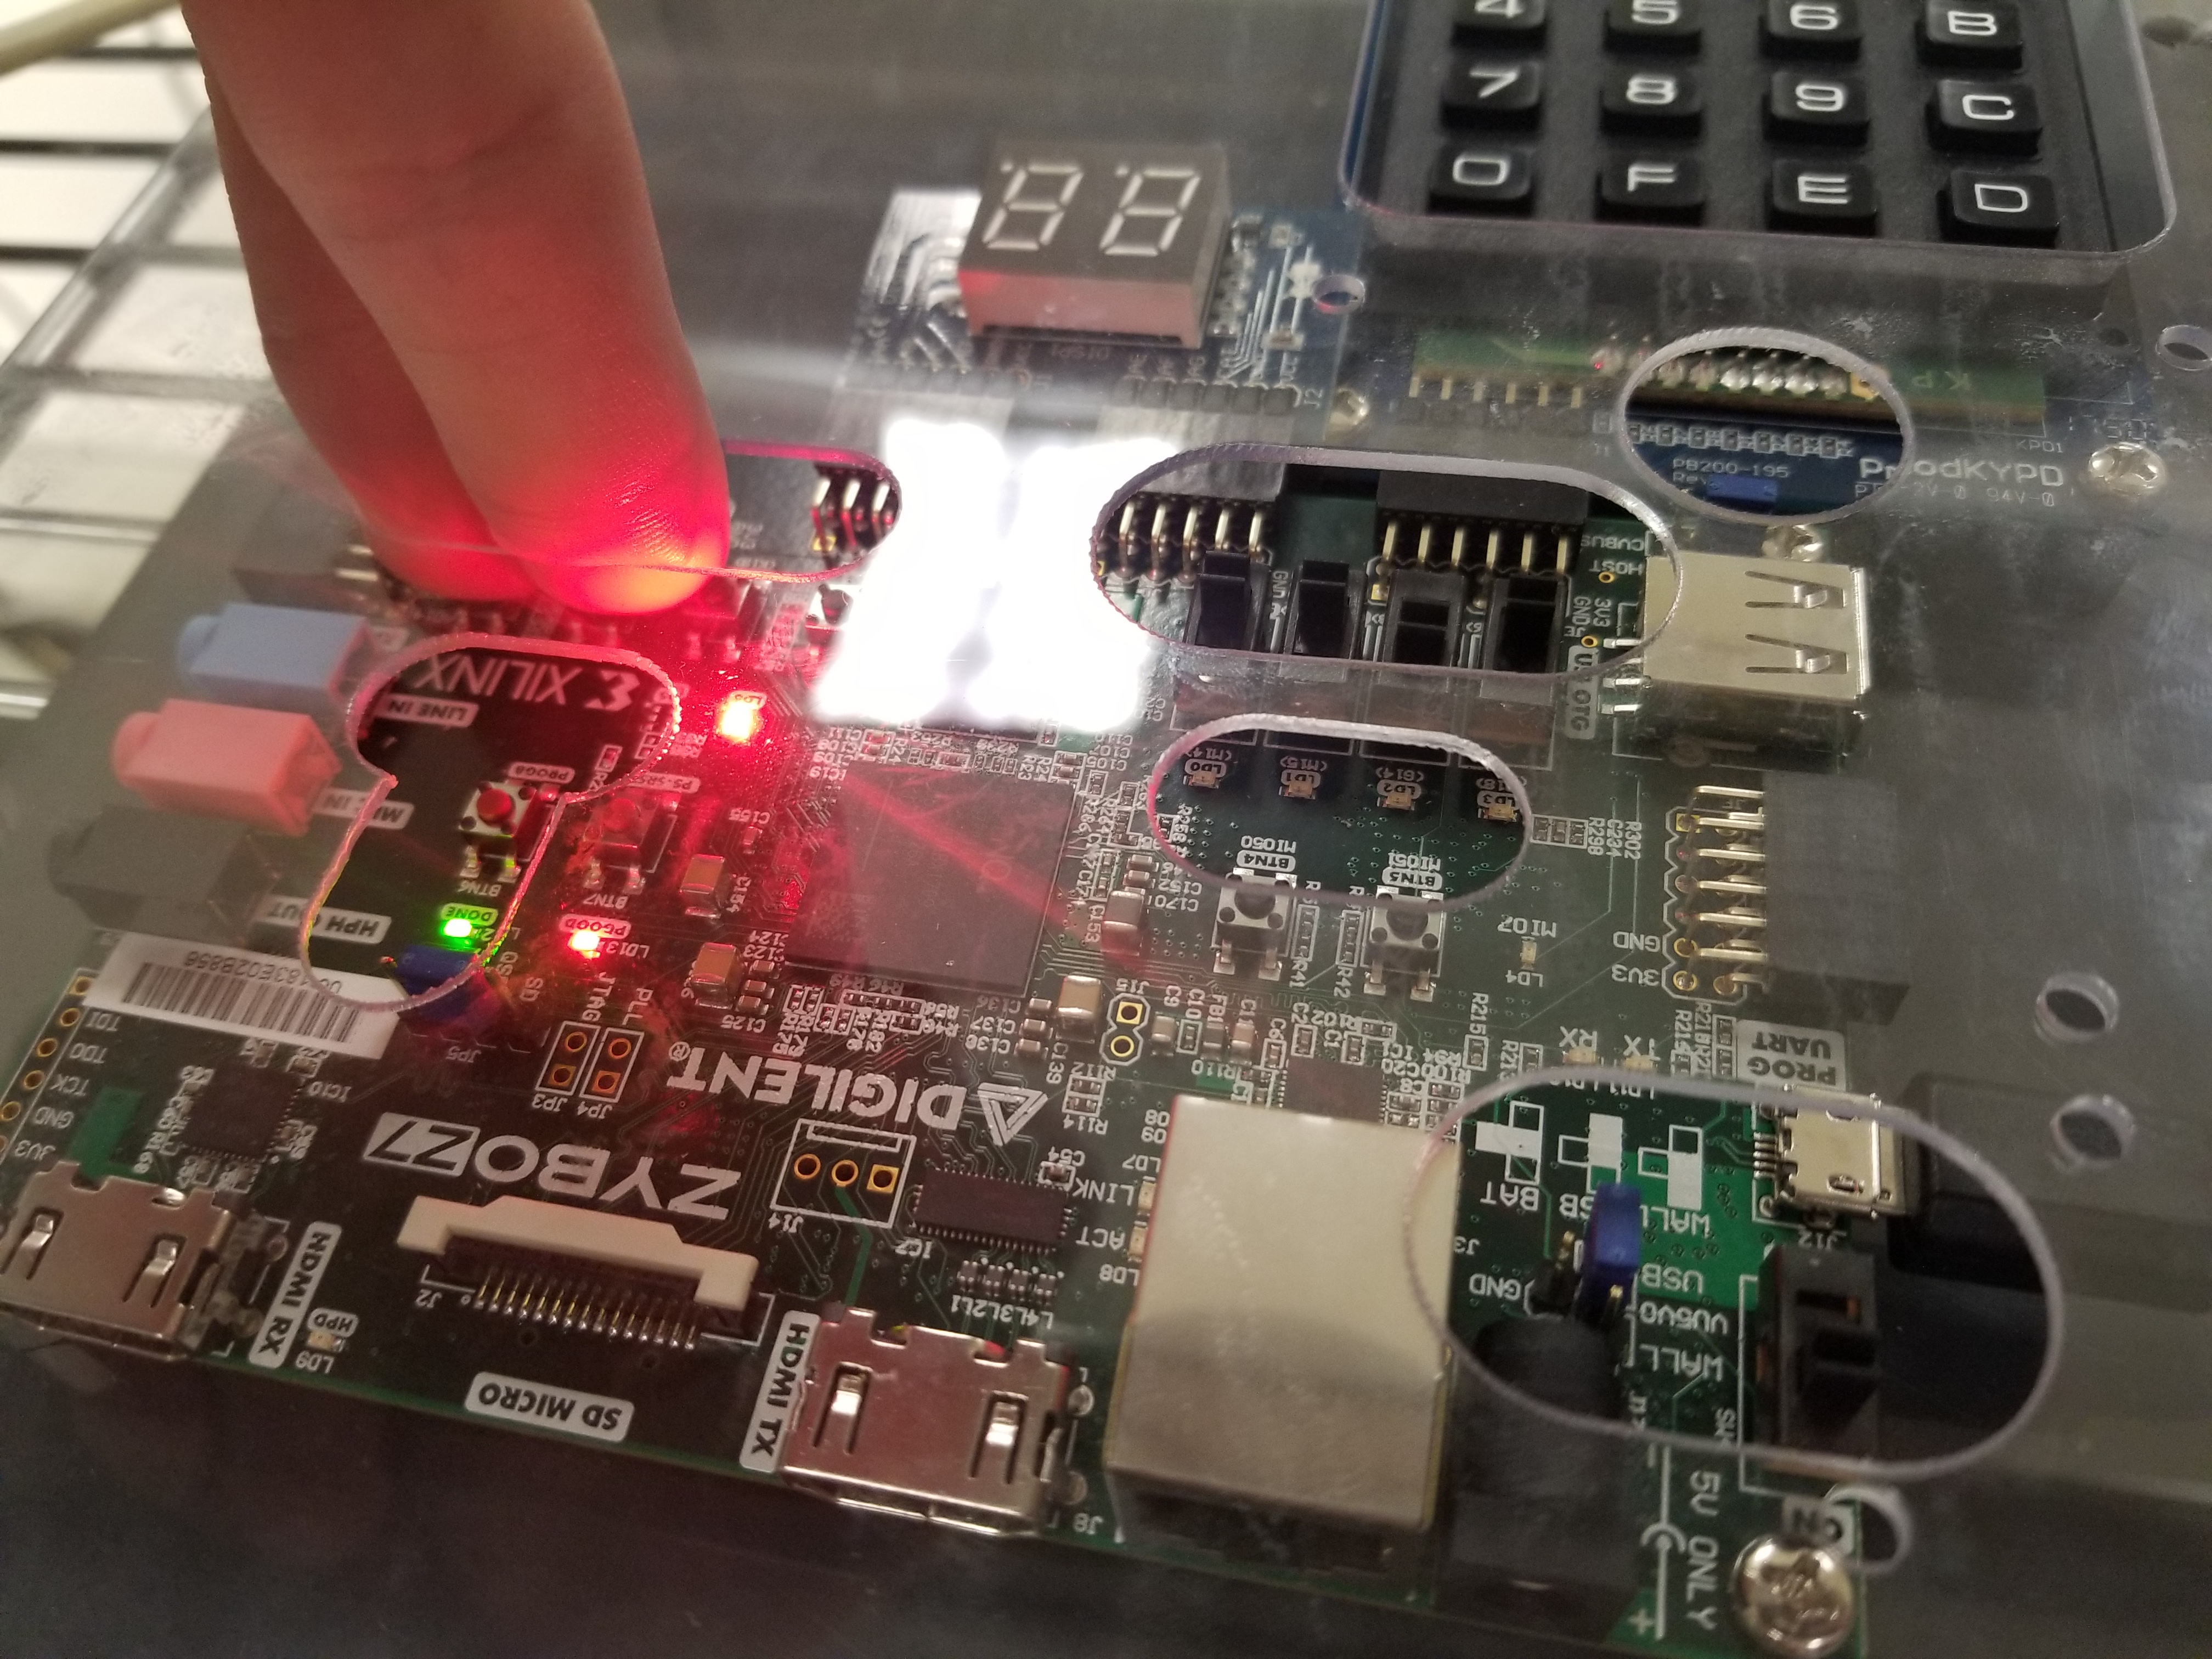
\includegraphics[width=\linewidth]{access_testing.jpg}
        \caption{Part 2 Physical Testing}
        \label{fig:part2_testing}
    \end{figure}


    \section{Discussion}
    Multiplexing and demultiplexing circuits are designed using 'selection' elements.
    These elements can also be repurposed to create functional
    and practical circuits for real life applications.
    
    \paragraph{Mux and Demux Circuit}

    \begin{enumerate}
            \item When the mux and demux select signals are in an unused state,
                There will be no signal outputs going to any of the engineers.
                
            \item Waveform can be found in the results section.

            \item The advantage of ICs is that you can physically see the layout of the circuit. As well, you can probe the internal connections.
                However, it is quite tedious to connect a large number of ICs together,
                and it can be quite error prone.
                The advantages of using an FPGA is that you can get a computer to make the connections for you.
                This allows you to rapidly design and prototype circuits. However, a disadvantage is that
                you cannot physically inspect the circuit and probe the internals.
    \end{enumerate}

    \paragraph{Lab Access Control}

    \begin{enumerate}
            \item The simulation waveform is provided above in the results section.

            \item I would rate the system as somewhat effective. However, it is not at all upgradable or expandable as designed.
                There are too few possible combinations, and these are set on toggle switches, which is not
                secure.
                It performs according to the given specifications.

            \item Something with a momentary keypad, as well as a programmable access control system.
                This would allow access to be given and revoked, passwords to be longer, and easily changable
                combinations.

    \end{enumerate}


    \section{Conclusion}
    Blinkies are cool.


\end{document}

